% Chapter 4: From Static to Contextual Embeddings

\section{Contextual Embeddings}

% Evolution to Contextual Embeddings
\begin{frame}{Evolution: From Static to Contextual Embeddings}
\textbf{The Next Revolution: Context Matters!}

\begin{columns}
\column{0.5\textwidth}
\textbf{Problem with Static Embeddings:}

One word = One vector always

\begin{center}
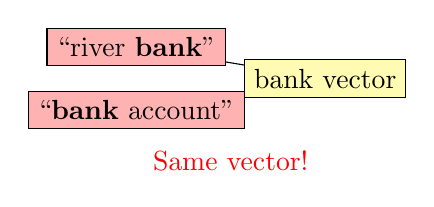
\begin{tikzpicture}[scale=0.8]
    \node[draw, fill=red!30] (bank1) at (0,1) {``river \textbf{bank}''};
    \node[draw, fill=red!30] (bank2) at (0,0) {``\textbf{bank} account''};
    
    \draw[->] (bank1) -- (3,0.5);
    \draw[->] (bank2) -- (3,0.5);
    
    \node[draw, fill=yellow!30] at (3,0.5) {bank vector};
    
    \node at (1.5,-0.8) {\textcolor{red}{Same vector!}};
\end{tikzpicture}
\end{center}

But ``bank'' has different meanings!

\vspace{0.3cm}
\textbf{Static Embedding Models:}
\begin{itemize}
    \item Word2Vec (2013)
    \item GloVe (2014)
    \item FastText (2016)
\end{itemize}

\column{0.5\textwidth}
\textbf{Solution: Contextual Embeddings}

Different contexts = Different vectors

\begin{center}
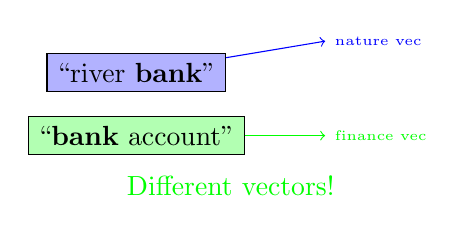
\begin{tikzpicture}[scale=0.8]
    \node[draw, fill=blue!30] (bank1) at (0,1) {``river \textbf{bank}''};
    \node[draw, fill=green!30] (bank2) at (0,0) {``\textbf{bank} account''};
    
    \draw[->, blue] (bank1) -- (3,1.5) node[right] {\tiny nature vec};
    \draw[->, green] (bank2) -- (3,0) node[right] {\tiny finance vec};
    
    \node at (1.5,-0.8) {\textcolor{green}{Different vectors!}};
\end{tikzpicture}
\end{center}

\textbf{Contextual Models:}
\begin{itemize}
    \item ELMo (2018) - RNN-based
    \item BERT (2018) - Transformer
    \item GPT (2018+) - Autoregressive
\end{itemize}

\textbf{Key Advance:}
Vector depends on surrounding words!
\end{columns}

\vspace{0.2cm}
\begin{center}
\colorbox{yellow!20}{\parbox{0.9\textwidth}{
\textbf{Evolution:} Static $\rightarrow$ Contextual = Major breakthrough in NLP!
}}
\end{center}
\end{frame}

% Summary and Applications
\begin{frame}{Summary: The Power of Embeddings}
\textbf{From Words to Understanding}

\begin{columns}
\column{0.5\textwidth}
\textbf{The Journey:}
\begin{center}
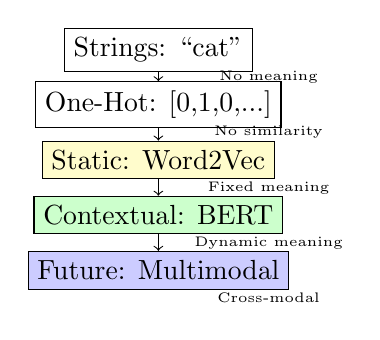
\begin{tikzpicture}[scale=0.7, node distance=1.5cm]
    \node[draw, rectangle] (strings) at (0,4) {Strings: ``cat''};
    \node[draw, rectangle] (onehot) at (0,3) {One-Hot: [0,1,0,...]};
    \node[draw, rectangle, fill=yellow!20] (static) at (0,2) {Static: Word2Vec};
    \node[draw, rectangle, fill=green!20] (context) at (0,1) {Contextual: BERT};
    \node[draw, rectangle, fill=blue!20] (future) at (0,0) {Future: Multimodal};
    
    \draw[->] (strings) -- (onehot);
    \draw[->] (onehot) -- (static);
    \draw[->] (static) -- (context);
    \draw[->] (context) -- (future);
    
    \node at (2,3.5) {\tiny No meaning};
    \node at (2,2.5) {\tiny No similarity};
    \node at (2,1.5) {\tiny Fixed meaning};
    \node at (2,0.5) {\tiny Dynamic meaning};
    \node at (2,-0.5) {\tiny Cross-modal};
\end{tikzpicture}
\end{center}

\column{0.5\textwidth}
\textbf{Applications Enabled:}
\begin{itemize}
    \item \textbf{Search:} Find similar documents
    \item \textbf{Translation:} Map between languages
    \item \textbf{Sentiment:} Understand emotions
    \item \textbf{QA:} Match questions to answers
    \item \textbf{Generation:} Create coherent text
\end{itemize}

\textbf{Key Insights:}
\begin{enumerate}
    \item Meaning can be encoded as vectors
    \item Similar words have similar vectors
    \item Relationships are directions
    \item Context changes everything
\end{enumerate}
\end{columns}

\vspace{0.3cm}
\begin{center}
\colorbox{blue!10}{\parbox{0.9\textwidth}{
\textbf{Remember:} Embeddings are the foundation of modern NLP - they turn words into numbers that capture meaning, enabling all downstream tasks!
}}
\end{center}

\textbf{Next Steps:} Experiment with pre-trained embeddings in your projects!
\end{frame}